\chapter[Used Software, Tools, etc.]{Used Software, Tools, etc.}%
\label{c:usedSoftware}%
This chapter provides an overview of the software and tools used to implement the Open3DScanner project. Furthermore used artefacts (libraries, 3D models, \dots) as well as the corresponding licenses are presented.%

The aim is to create an as complete as possible list of the dependencies of the Open3DScanner in order to have all relevant license information at one central location.%

Transitive dependencies, which result from the used artefacts, are excluded from the consideration. If you are interested, please refer to the documentation of the respective artifact, which is linked at the appropriate place of this document, if available.%

\section{Arduino}%
Since the heart of the Open3DScanner is an ESP32\sideNote[white]{Detailed information about the ESP32, including its data sheet, can be found on the \hrefIdx{https://www.espressif.com/en/products/hardware/esp32/overview}{Espressif ESP32 product page}.} and the development should be done with the \hrefIdx{https://www.arduino.cc/en/main/software}{Arduino IDE}, one of the most important dependencies in the Arduino area is the {\faGithub} \hrefIdx{https://github.com/espressif/arduino-esp32}{Arduino core for ESP32 WiFi chip}, which allows the use of ESP32 development boards with the Arduino IDE. This simplifies the development of the project considerably.%

The Arduino IDE is released under the GPL license, while the included libraries are released under the LGPL license. The LGPL license is also applied to the Arduino core for the ESP32 WiFi chip.%

\subsection{Libraries}%
In the following the libraries which were used for the implementation of the Open3DScanner and are not included in the Arduino IDE are described.%

\begin{table}[ht!]%
	\begin{centered}%
		\rowcolors{2}{tableLineTwo}{tableLineOne}% specify rowcolors in tabularx style
		\begin{tabularx} {\linewidth} {>{\rowmac \hsize=1.3\hsize}X>{\rowmac \hsize=0.5\hsize}X>{\rowmac \hsize=0.9\hsize}X>{\rowmac \hsize=0.8\hsize}X>{\rowmac \hsize=1.5\hsize}X<{\clearrow}}%
			\tabularxHeader%
			Library & Version & Author & License & Purpose\\%
			{\faGithub} \hrefIdx{https://github.com/platisd/nokia-5110-lcd-library}{nokia-5110-lcd-library} & 2.0.0 & platisd & MIT License & Driving the Nokia 5110 LCD.\\%
			{\faGithub} \hrefIdx{https://github.com/laurb9/StepperDriver}{StepperDriver} & 1.1.4 & laurb9 & not specified & Two-pin stepper motor driver library.\\%
			{\faGithub} \hrefIdx{https://github.com/madhephaestus/ESP32Encoder/}{ESP32Encoder} & 0.1.5 & madhephaestus  & MIT License & Rotary encoder library using interrupts.\\%
			{\faGithub} \hrefIdx{https://github.com/jonblack/arduino-menusystem}{arduino-menusystem} & 3.0.0 & jonblack & MIT License & Ddata structures for menu structures.\\%
		\end{tabularx}%
		\caption{Arduino Libraries used within the Open3DScanner}%
	\end{centered}%
\end{table}%

It can be seen that only a few external libraries are required in total, since a large part of the functionality is already available through the libraries provided by the Arduino IDE and the Arduino core for ESP32 WiFi chip.%

\marginElement{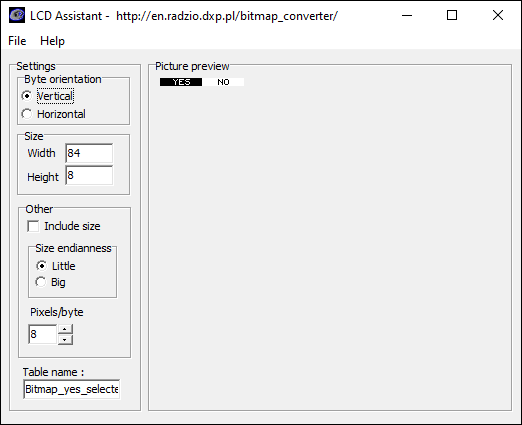
\includegraphics[width=\linewidth]{images/LCDAssistant.png}\captionof{figure}{LCDAssistant GUI}}%

In some places the display of the Open3DScanner shows other things as pure text, e.g. to show buttons. For this purpose, corresponding bitmaps were created, which were then translated into corresponding character arrays with the tool \hrefIdx{http://en.radzio.dxp.pl/bitmap_converter/}{LCD Assistant}\marginInfo[LCDAssistant]{The LCDAssistant is a useful tool that allows the easy transformation of bitmaps into character arrays, which can directly fed to the various LCD screens. It provides some configuration to match different LCDs.} from Radosław Kwiecień.%

The license of the LCD Assistant is not specified by the developer on the project page.%

\section{Schematics and PCB Design}%
Although it is practical to test the necessary circuits on a solderless breadboard during development, this is not a long-term solution. This is especially true if you consider that the breadboard creates new sources of error.%

In addition to the generally known problems, such as instability (in general, but also with e.g. vibrations) and high space requirements compared to a custom PCB, it must be noted that the individual tracks of the breadboard have high resistances and can introduce unwanted capacitances into the circuit\sideNote{More information about unwanted side effects that can occur when using breadboards can be found on \hrefIdx{https://hackaday.com/2016/01/19/solderless-breadboard-parasitics/}{Hackaday} and \hrefIdx{https://breadboardadventures.com/2016/02/14/a-square-and-triangle-wave-vco-part-ii-taming-the-voltage-spikes/}{Breadboard Adventures}.}.%

During development it was not possible to use an LDO\sideNote{Low Dropout} regulator on the breadboard and to get a stable output voltage of \SI{5}{\volt}. Instead it was necessary to outsource the low-dropout and its components to a prototype PCB to get a stable output voltage. Otherwise, it would not have been possible to test the circuit design, as spontaneous voltage drops led to crashes of the ESP32.%

Figure~\ref{f:breadboard} shows the circuit of the Open3DScanner on a breadboard. In addition the prototype PCB with the LDO regulator is visible. It's easy to see that the circuit is chaotic and therefore difficult to maintain, debug, and develop. For the picture even cables have been removed: The stepper motors are not connected and the lights have been removed.%

Due to the size of the components it was necessary to use two breadboards, which makes the whole construction extremely fragile. More than 50 cables were needed to build the circuit on the breadboards.%

\begin{figure}[ht!]%
	\begin{centered}%
		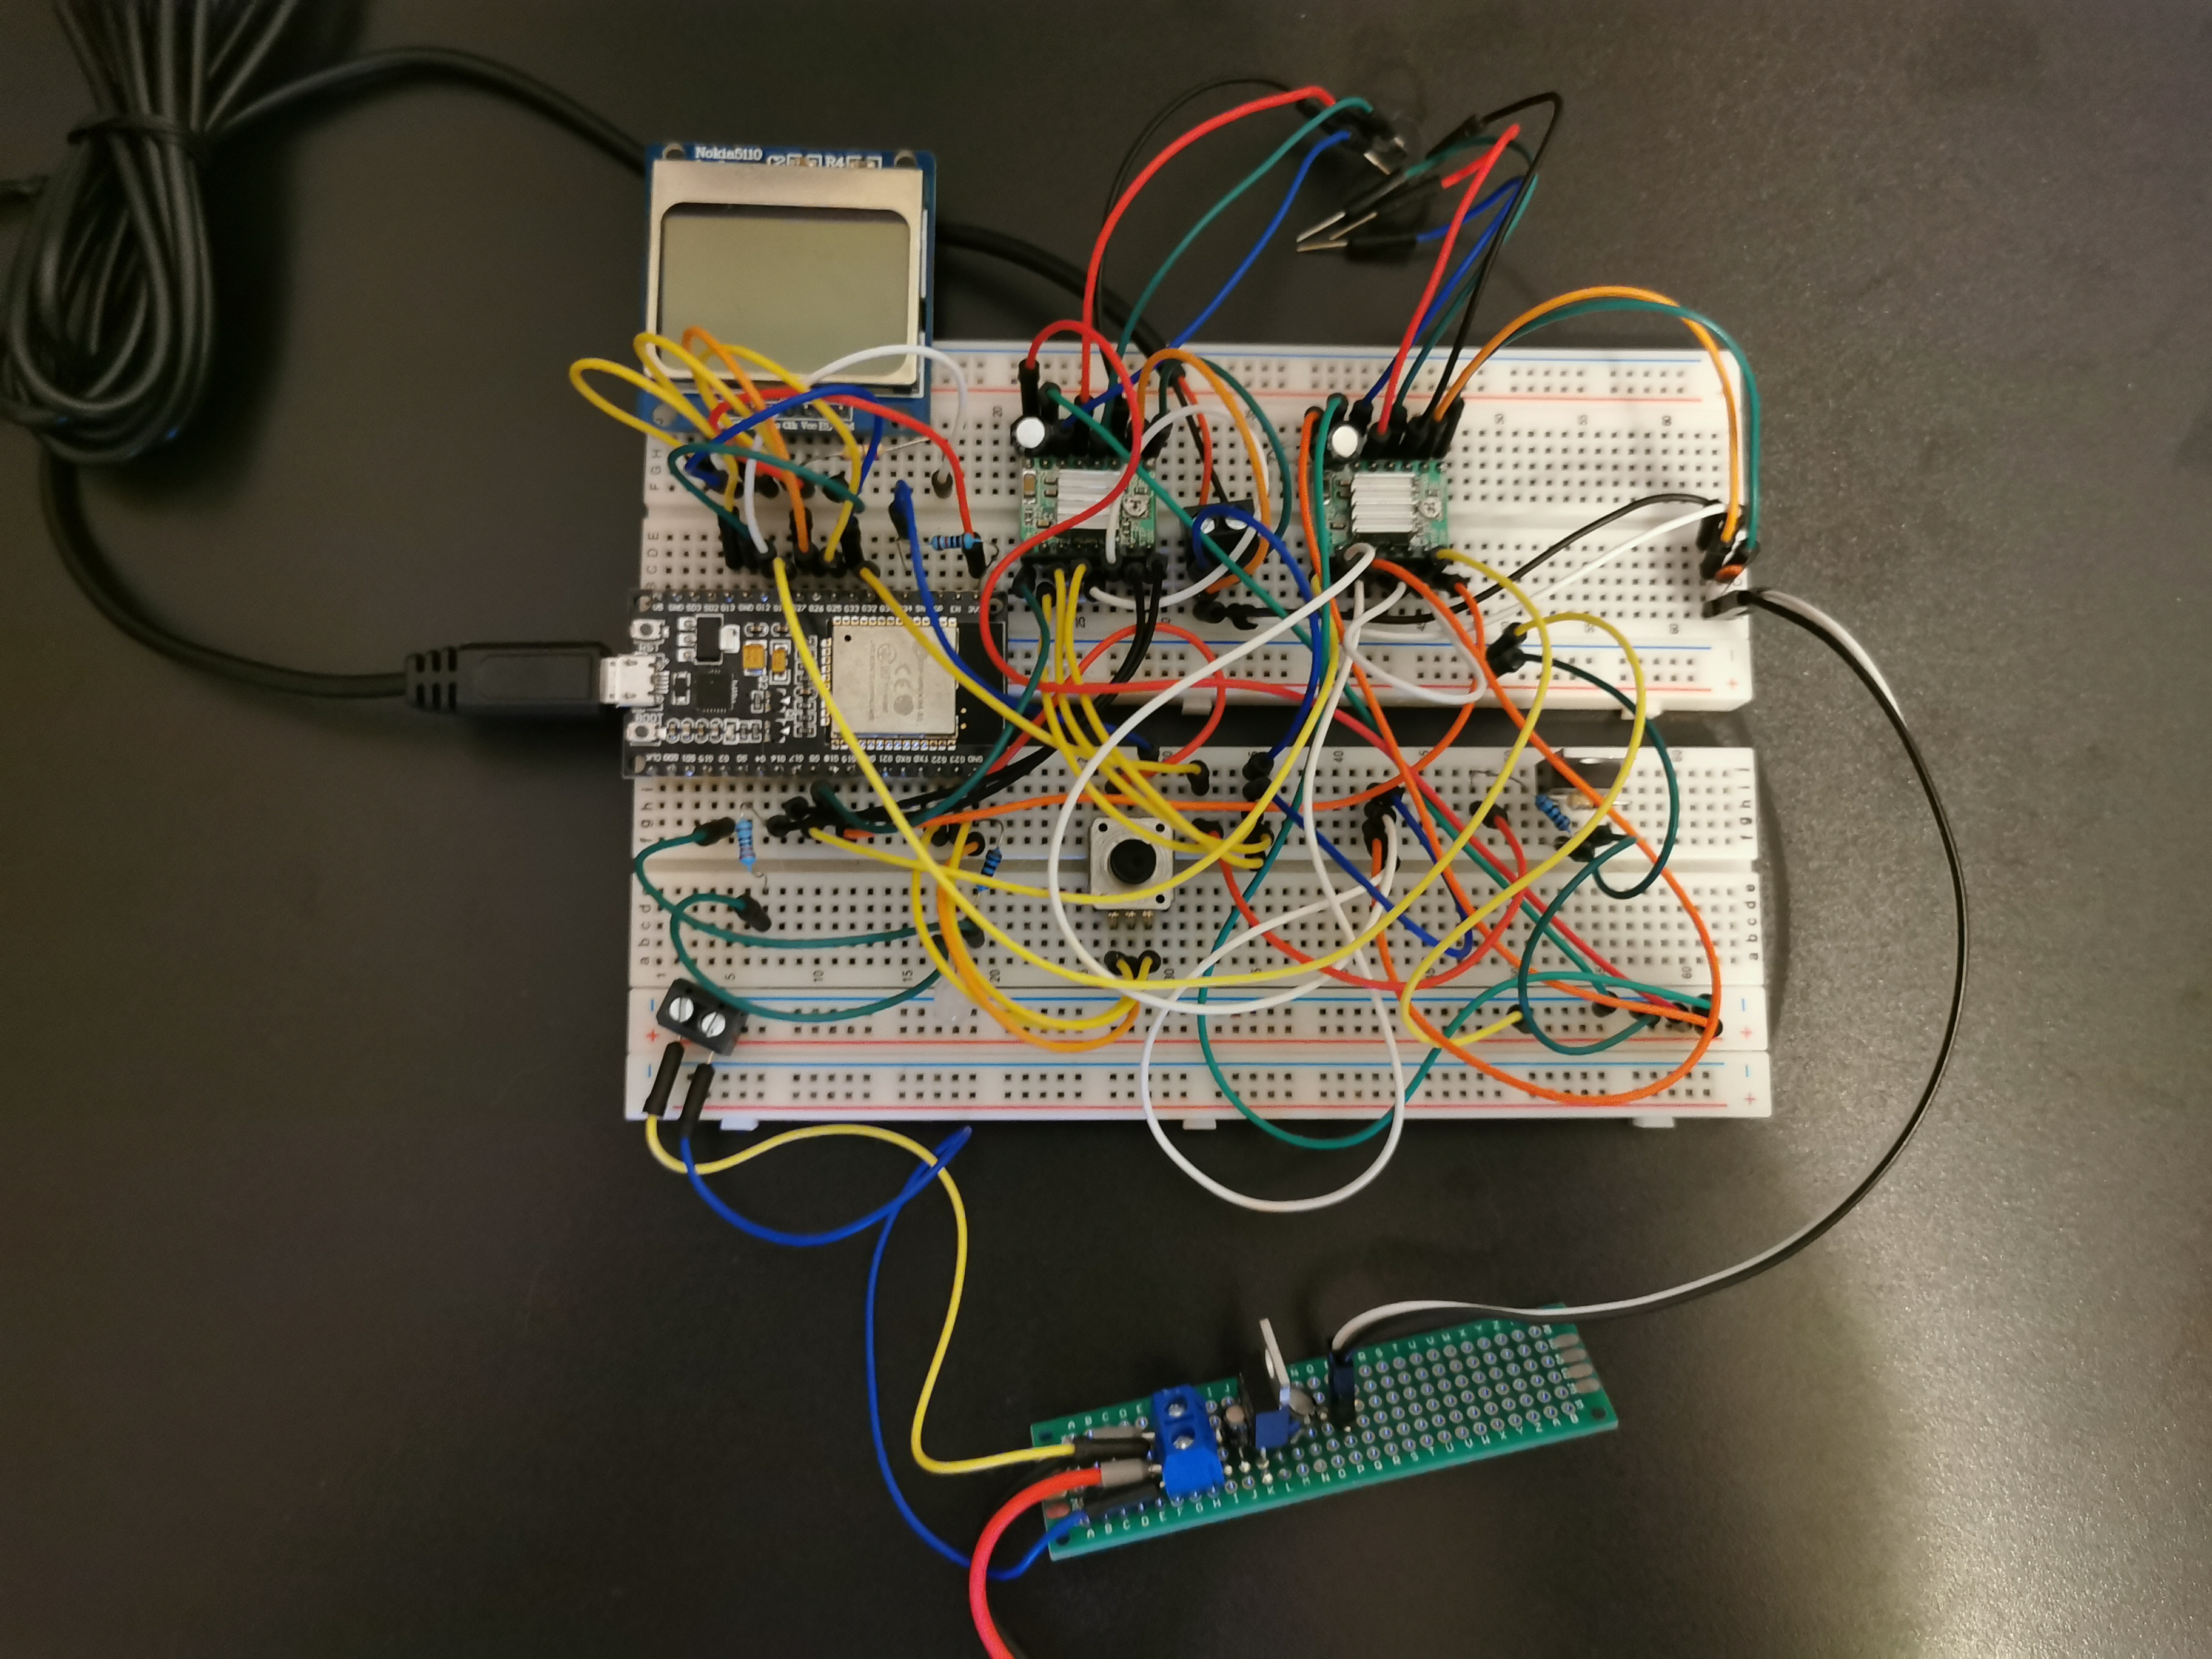
\includegraphics[width=\linewidth]{images/Breadboard.jpg}%
		\caption{The Open3DScanner circuit on a solderless Breadboard}%
		\label{f:breadboard}%
	\end{centered}%
\end{figure}%

It quickly becomes clear that in the long run it is necessary to design and manufacture\marginTips[JLCPCP]{The PCBs for the first prototype of the Open3DScanner were manufactured by \hrefIdx{https://jlcpcb.com/}{JLCPBP}. The manufacturer is located in China and offers very cheap PCBs, which were of very good quality when I ordered them. The only disadvantage, besides the minimum order of 5 boards, is that even the fastest shipping takes about a week. However, this is more than compensated when comparing prices with local suppliers.} a special PCB for the Open3DScanner.%

For the design of the board the software \hrefIdx{http://www.kicad-pcb.org/}{KiCad} was used.  KiCad is an open source program package licensed under the GPL.%

KiCad contains tools for all steps involved in designing a PCB. The individual tools offer very good integration with each other, which simplifies the design process considerably.%

First you create a schematic diagram for the circuit. The individual components are connected with so-called footprints. These footprints define the layout of the individual components on the board (holes, labels, \dots). With this information you go over to the actual design of the PCB. Figure~\ref{f:schematic} shows the schematic diagram for the Open3DScanner.%

\begin{figure}[ht!]%
		\sideCaptionOfL{figure}{Schematic diagram for the Open3DScanner designed in KiCad}{f:schematic}%
		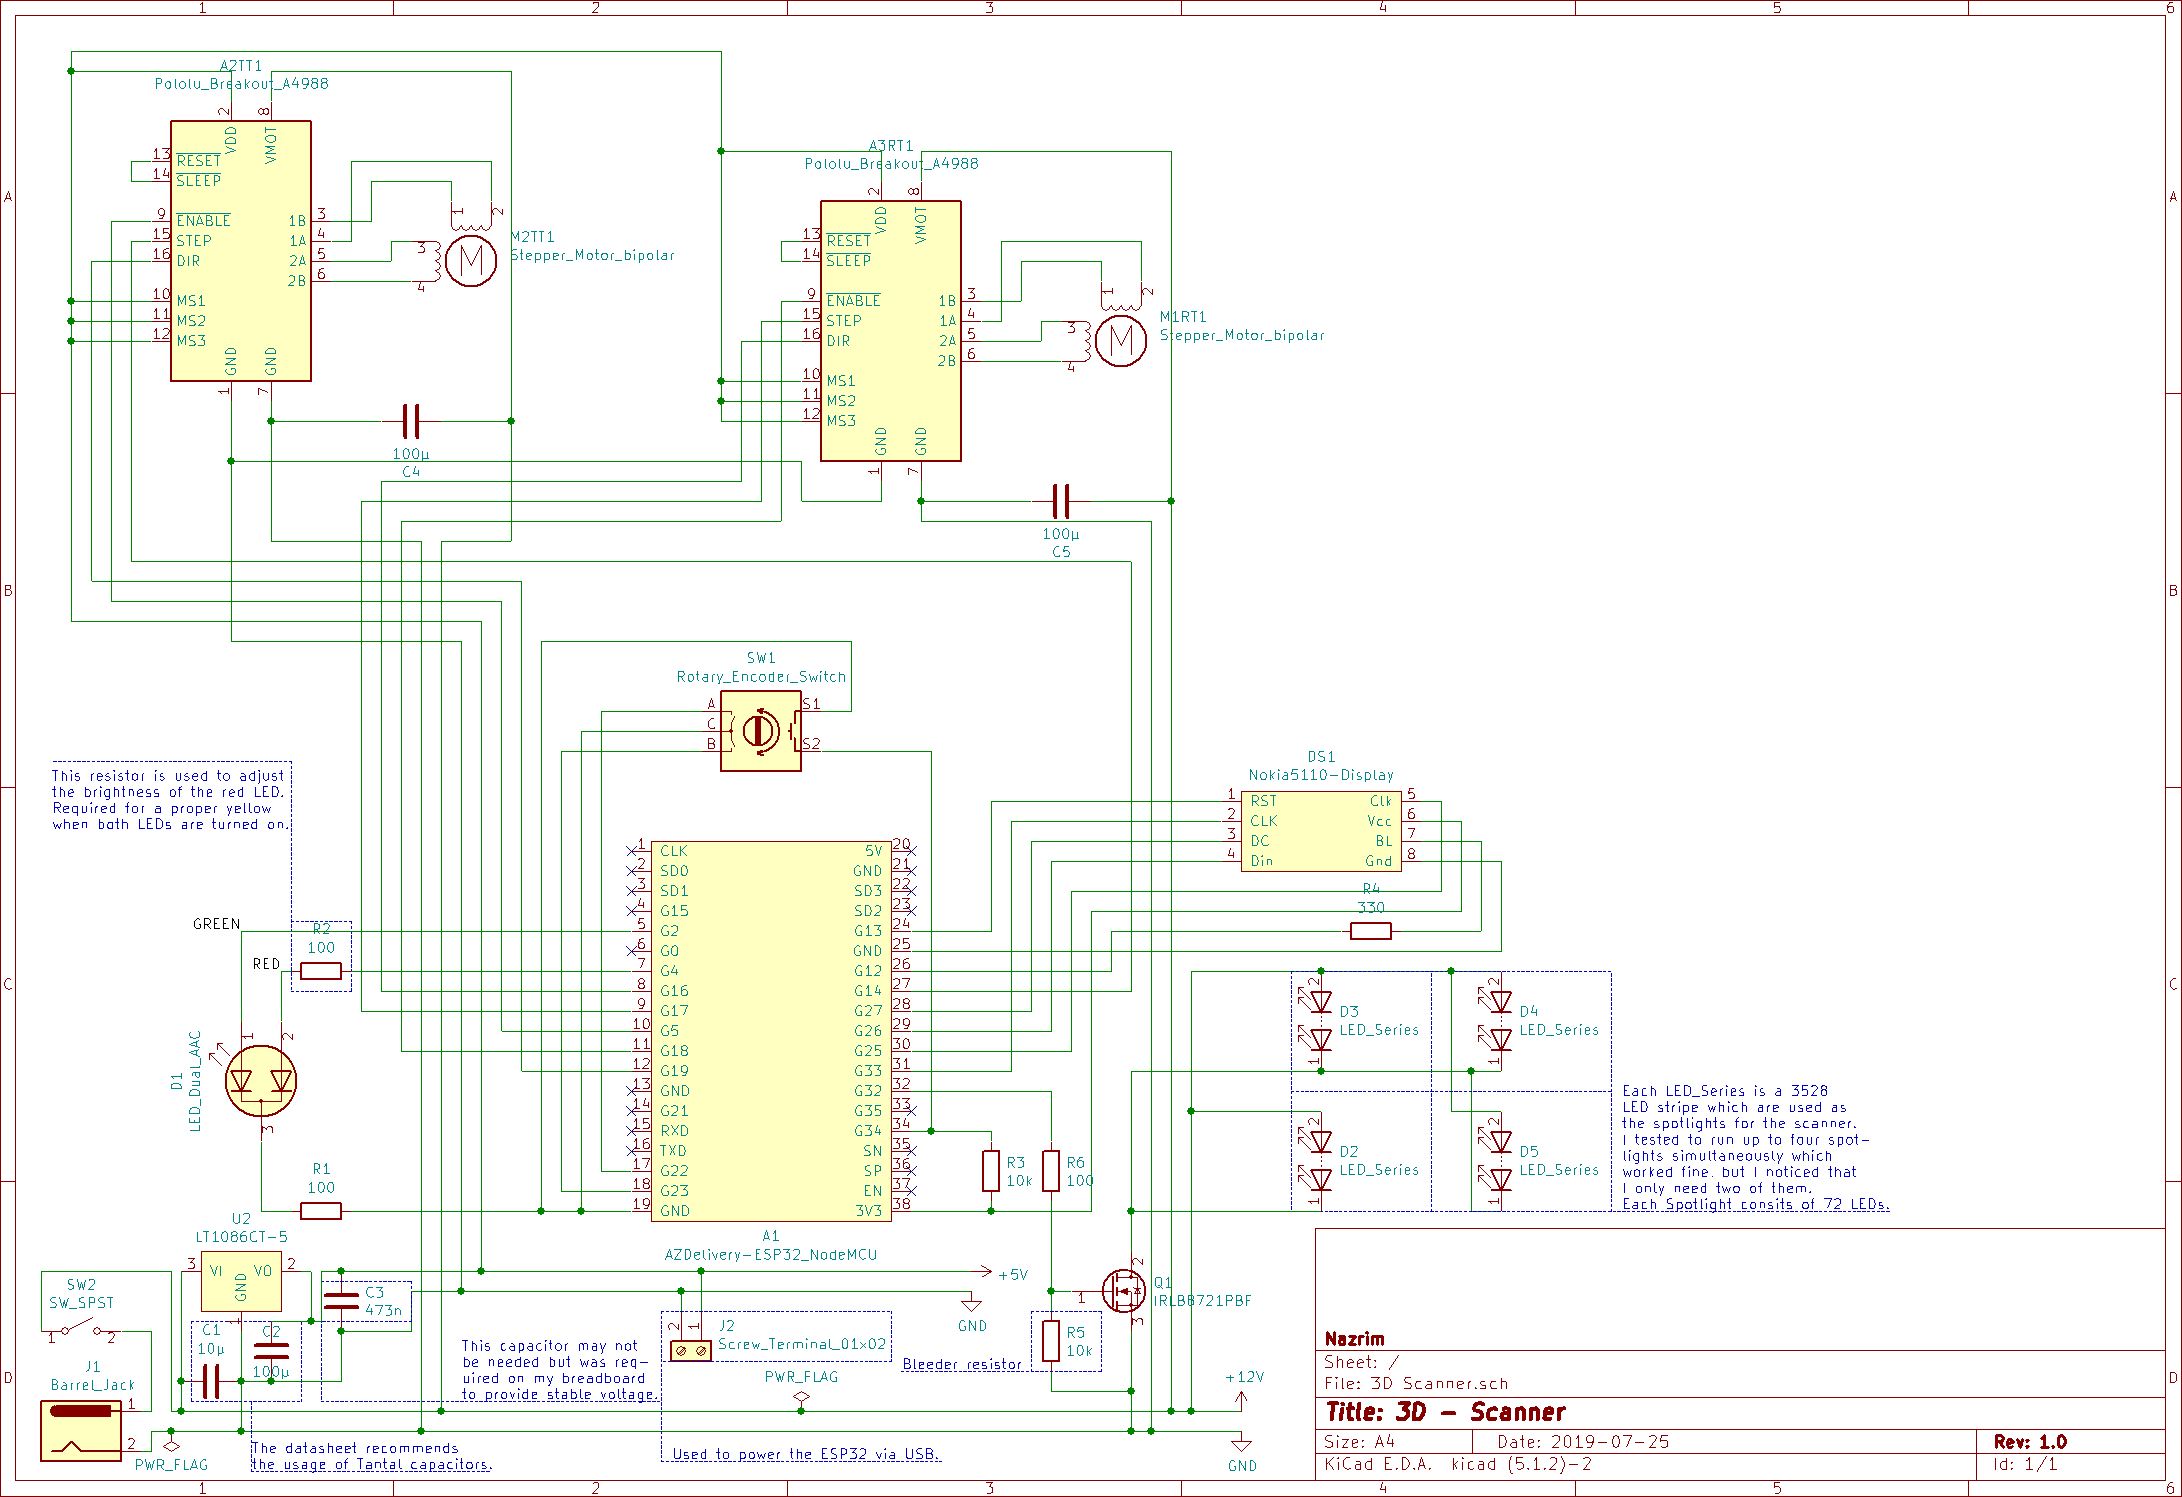
\includegraphics[width=\linewidth]{images/Schematic.png}%
\end{figure}%


All elements are placed on an empty surface, which represents the later board. The user now has to position the individual elements and draw traces for the connections. The user is always shown which pins have to be connected to each other. Figure~\ref{f:pcb} shows the PCB design for the Open3DScanner.%

\begin{figure}[ht!]%
		\sideCaptionOfL{figure}{PCB design for the Open3DScanner designed in KiCad}{f:pcb}%
		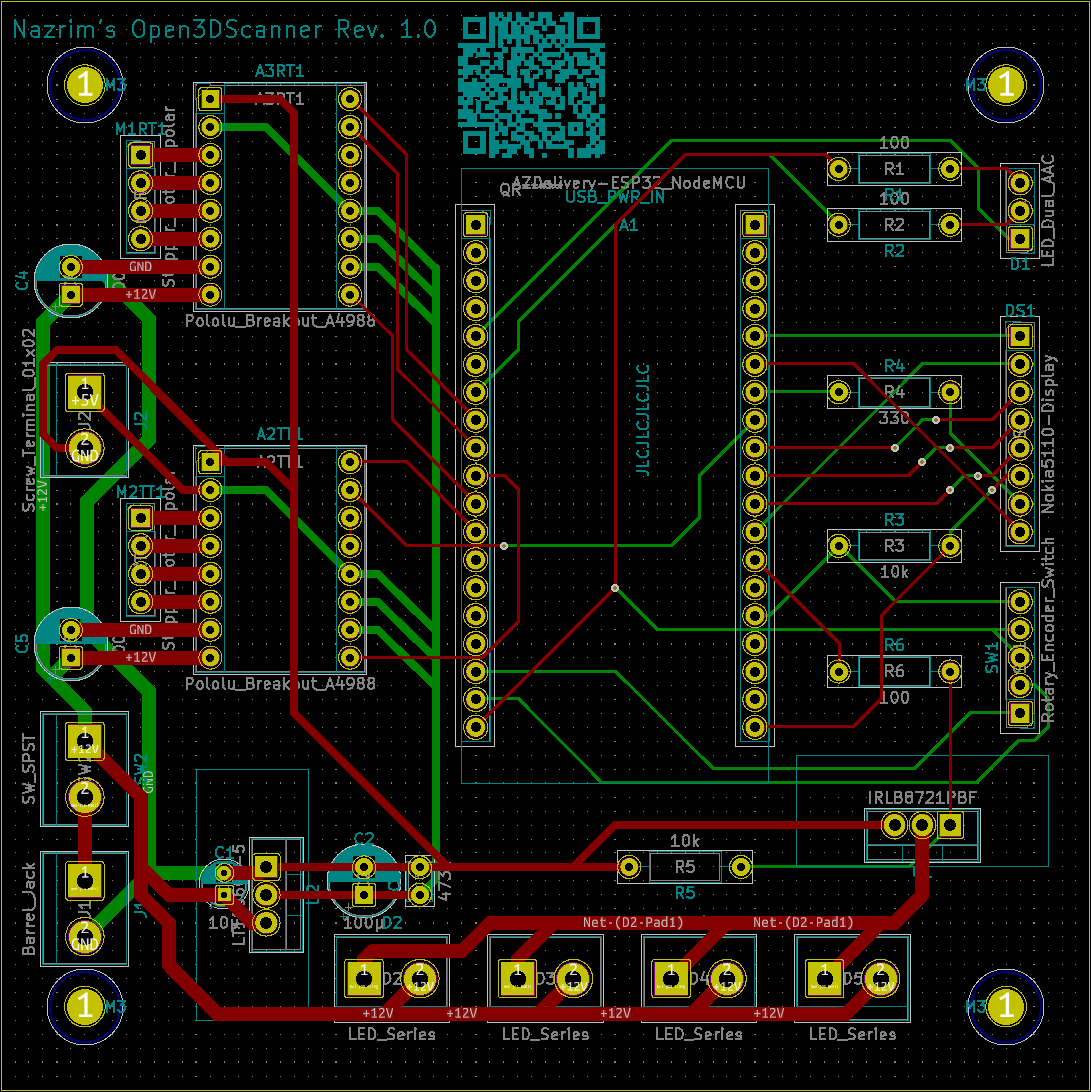
\includegraphics[width=\linewidth]{images/PCB.png}%
\end{figure}%

At this point all necessary steps for the design of the PCB are completed. The necessary Gerber files\marginInfo[Gerber Files]{Manufacturers generally provide instructions on which Gerber files to use and which naming conventions to follow. Often there are even instructions for concrete software.} can be generated and handed over to an appropriate service provider for production.%

Alternatively, a 3D model of the finished board (with all components) can be created beforehand. For this it is necessary to link the footprints with 3D models. For the rendering of the 3D model no further effort is necessary.%

I consider this step very useful. On the one hand you get a better idea of what the finished board will look like and on the other hand you can check again that no components are in conflict with each other. This is especially important in case of a high packing density of the components. Figure~\ref{f:render} shows the rendered 3D model of the Open3DScanner's board including all components.%

\begin{figure}[ht!]%
	\sideCaptionOfL{figure}{3D rendering of the PCB including components for the Open3DScanner designed in KiCad}{f:render}%
	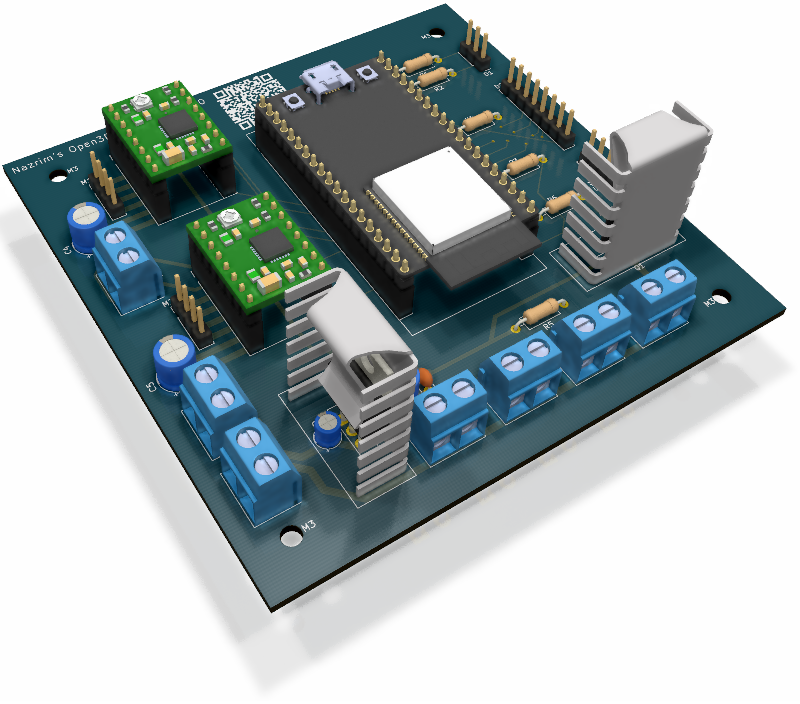
\includegraphics[width=\linewidth]{images/Render.png}%
\end{figure}%

Due to the large number of existing components, KiCad cannot contain a schematic symbol, footprint, and 3D model for all of them. It is also possible that a different footprint should be selected for a component, for example because it is not connected directly to the board, but via a pin header.%

This also applied to several parts of the Open3DScanner. In case of missing schematic symbols and footprints, it is possible to draw the corresponding parts via intuitive integrated editors.%

If 3D models for components are missing, it is necessary to provide them (for example as STEP file). If this does not happen, the board can still be rendered, but the corresponding part locations remain empty.%

A possible source for corresponding 3D models of components to be used in open source projects is  \hrefIdx{https://grabcad.com/library}{GrabCAD}\marginCritical[GrabCAD License]{3D models obtained from GrabCAD may only be used for non-commercial purposes. For commercial use, permission must be obtained from the author of the model.}. For licensing reasons I prefer other sources for obtaining 3D models of components. On the one hand many manufacturers already provide corresponding CAD files and on the other hand \hrefIdx{https://www.snapeda.com/}{SnapEDA} offers a large database of components containing a schematic symbol, a PCB footprint, and a 3D model. The individual entries are licensed under CC-BY-SA 4.0.%

\subsection{Used 3D Models}%
This section lists the 3D models which are not already part of KiCad and which are used to render the Open3DScanner board and their source.%

\begin{table}[ht!]%
		\sideCaptionOf{table}{3D Models used for rendering the Open3DScanner}%
		\rowcolors{2}{tableLineTwo}{tableLineOne}% specify rowcolors in tabularx style
		\begin{tabularx} {\linewidth} {>{\rowmac \hsize=\hsize}X>{\rowmac \hsize=\hsize}X<{\clearrow}}%
			\tabularxHeader%
			Component & Source\\%
			ESP32 Devkit-C  & \href{https://www.snapeda.com/parts/ESP32-DEVKITC-32D/Espressif\%20Systems/view-part/}{SnapEDA - ESP32-DEVKITC-32D}\\%
			Blue two pole screw terminal & \hrefIdx{https://www.snapeda.com/parts/TB002-500-02BE/CUI\%20Inc./view-part/}{SnapEDA - TB002-500-02BE}\\%
			A4988 stepper driver & \hrefIdx{https://www.pololu.com/product/1182}{Pololu - A4988 product page}\\%
			TO 220 attachable heatsink & \hrefIdx{https://www.fischerelektronik.de/web\_fischer/en\_GB/heatsinks/C02/Attachable\%20heatsink/PG/FK245MI247O/search.xhtml}{fischer elektronik - FK 245 MI 247 O product page}\\%
		\end{tabularx}%
\end{table}%

\section{3D Design}%
When it comes to the 3D modeling of the Open3DScanner, there is little special to mention.%

\marginElement{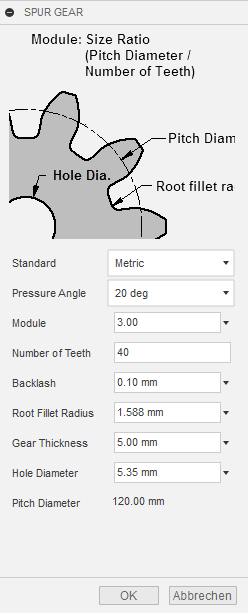
\includegraphics[width=\linewidth]{images/Spur_gear_3d_scanner_gear.png}\captionof{figure}{Fusion 360 script settings for creating the Open3DScanner's spur gear}}%

All components needed for the project and printed with a 3D printer were designed with \hrefIdx{https://www.autodesk.de/products/fusion-360/overview}{Fusion 360}. It should be noted that Fusion 360 contains handy scripts to create certain elements automatically. One of these scripts allows the creation of gears with given parameters. This script was used for the gears in the Open3DScanner.%

CAD models of some standard components such as ball bearings are required for the subsequent building instructions and render images of the finished Open3DScanner.%

\begin{table}[ht!]%
	\rowcolors{2}{tableLineTwo}{tableLineOne}% specify rowcolors in tabularx style
	\begin{tabularx} {\linewidth} {>{\rowmac \hsize=1.2\hsize}X>{\rowmac \hsize=0.9\hsize}X>{\rowmac \hsize=0.9\hsize}X<{\clearrow}}%
		\tabularxHeader%
		Source & Model Type & License\\%
		\hrefIdx{https://www.astbearings.com/free-3d-cad-models-for-bearings.html}{AST Bearings} & Bearings & not specified, but free\\%
		\faGithub{} \hrefIdx{https://github.com/Hecatron-Machines/Cad.Solidworks.Parts}{Cad.Solidworks.Parts}& Nema 17 & MIT\\%
		\hrefIdx{https://octopart.com/terms}{Octopart} & Various & not specified, but free\\%
		\faGithub{} \hrefIdx{https://github.com/FreeCAD/FreeCAD-library}{FreeCAD-library}& Dupont Connectors & CC-BY 3.0\\%
		\hrefIdx{https://www.digikey.de//resources/3d-models}{Digi-Key}& Molex Connectors \& Cable Lugs & not specified, but free\\%
		\hrefIdx{https://www.snapeda.com/}{SnapEDA}& Micro USB-B Connector & CC-BY-SA 4.0\\%
	\end{tabularx}%
	\caption{Sources for CAD models of non-electrical components}%
	\label{t:cad}%
\end{table}%

There are several vendors with large libraries of CAD models, which may not be freely used and/or distributed. Table~\ref{t:cad} contains information which offers were used for which models.%

\section{Photogrammetry}%
\label{sec:photogrammetry}
The heart of the entire photogrammetry process is the software that creates the 3D model from the images taken.%

For this purpose I use the software \hrefIdx{https://alicevision.org/\#meshroom}{Meshroom}. It is intuitive to use and performs the entire process. The finished (textured) 3D model is created from the fed-in images. Alternative software solutions do not always offer the entire process and generate for example only a point cloud, which has to be converted into a 3D model with another program. This applies for example to \hrefIdx{http://ccwu.me/vsfm/}{VisualSFM}.%

Meshroom is released under the MPL 2.0 and can be compiled by the user or can be obtained as a ready-to-use installer.%

In general, I would recommend the use of Meshroom to anyone, simply because it is very easy to use and produces great results while offering extensive configuration options.%

The only limitation is that a CUDA-enabled graphics card (Nvidia) is required for optimal results, as the calculations are done on the GPU. If such a card is not available, a "preview mode" can be activated, which works without CUDA, but also produces worse results.%

\section{\LaTeX}%
\LaTeX{} was used to create this manual and last but not least we will look at which packages were used to create it.%

The document class used is yReport from Harvey Sheppard. The class is part of his project {\faGithub} \hrefIdx{https://github.com/HarveySheppard/yLaTeX}{yLatex}, which provides document classes and packages to create appealing documents. The entire yLatex project is licensed with LPPL 1.3.%

The compiler used is \hrefIdx{http://www.tug.org/xetex/}{\hologo{XeLaTeX}}, which is required by the document class yReport. \hrefIdx{https://www.tug.org/texlive/}{\hologo{TeX} Live} is used as \hologo{TeX} distribution and \hrefIdx{https://www.texstudio.org/}{\hologo{TeX}studio} as editor.%

Pictures can be found in various places in this document. If these images are not photos, screenshots, or exports from other software, the images were created with Gimp which is licensed under the GPL.%

In addition, various packages are used to realize individual aspects of the document. These are listed below.%

\begin{table}[ht!]%
	\begin{centered}%
		\rowcolors{2}{tableLineTwo}{tableLineOne}% specify rowcolors in tabularx style
		\begin{tabularx} {\linewidth} {>{\rowmac \hsize=1.0\hsize}X>{\rowmac \hsize=0.7\hsize}X>{\rowmac \hsize=1.0\hsize}X>{\rowmac \hsize=0.5\hsize}X>{\rowmac \hsize=1.8\hsize}X<{\clearrow}}%
			\tabularxHeader%
			Package & Version & Maintainer & License & Purpose\\%
			\hrefIdx{https://ctan.org/pkg/fontawesome}{fontawesome5}  & 5.9.0 & Marcel Krüger & LPPL 1.3c \& OFL & Required by yAuthorBlock and used to show some icons across the document.\\%
			{\faGithub} \hrefIdx{https://github.com/HarveySheppard/yLaTeX}{yAuthorBlock}  & unknown & Harvey Sheppard & LPPL 1.3 & Used to create the author block on the second page.\\%
			\hrefIdx{https://ctan.org/pkg/tabularx}{tabularx}  & 2.11 & The \LaTeX{} Team & LPPL 1.3 & Since tabu (used by yReport) is somewhat buggy, this document uses tabularx.\\%
			\hrefIdx{https://ctan.org/pkg/siunitx}{siunitx}  & 2.7s & Joseph Wright & LPPL 1.3c & Used to display numbers and units in a proper way.\\%
			\hrefIdx{https://ctan.org/pkg/indextools}{indextools}  & 1.5.1 & Maïeul Rouquette & LPPL 1.3 & Used to build an index of all weblinks for printed documents.\\%
			\hrefIdx{https://ctan.org/pkg/xparse}{xparse} & 2019-05-28 & The \LaTeX{} Team & LPPL 1.3c & Required for string magic to display urls in the index (Appendix~\ref{ca:refs}) in a proper way.\\%
			{\faGithub} \hrefIdx{https://github.com/HarveySheppard/yLaTeX}{infoBulle}  & unknown & Harvey Sheppard & LPPL 1.3 & Used for displaying various block types (info, warning, \dots) in main area.\\%
			{\faGithub} \hrefIdx{https://github.com/HarveySheppard/yLaTeX}{marginInfoBulle}  & unknown & Harvey Sheppard & LPPL 1.3 & Used for displaying various block types (info, warning, \dots) in margin area.\\%
			\hrefIdx{https://ctan.org/pkg/isodate}{isodate}  & 2.28 & Harald Harders & LPPL 1.3c & Used for uniform displaying dates. Required because of strange behaviour of datetime package (included in yReport).\\%
			\hrefIdx{https://ctan.org/pkg/xurl}{xurl}  & 0.07 & Herbert Vo\ss{} & LPPL 1.3 & Allow URL breaks at any alphanumerical character.\\%
			\hrefIdx{https://ctan.org/pkg/hologo}{hologo}  & 1.13 & Heiko Oberdiek & LPPL 1.3 & Used to disaplay logos from the \LaTeX{} family.\\%
		\end{tabularx}%
		\caption{Used \LaTeX{} packages within the Open3DScanner's manual}%
	\end{centered}%
\end{table}%
